\chapter*{Results}
\label{ch:results}
% The performances of the models were evaluated using the
% \texttt{classification\_report} function from the \texttt{scikit-learn} library. 
% This function is particularly useful as it offers an overview of key evaluation
% metrics commonly used in Machine Learning, i.e. accuracy, precision, recall,
% and F1-score.\\
The performance metrics taken into account for evaluation are the following:
accuracy, precision, recall, and F1-score. Taking all of them into account
is crucial to accurately evaluate how well each model performs.

For the static models implemented in this project, the classification report
revealed an accuracy of 34\% for the Random Forest algorithm and 43\% for SVM. 
These results can be considered reasonable, given that the task at hand is a
multi-class classification problem with 8 classes.\\

Neural Networks' performances were generally not on par with the ones obtained by
the static models.
As mentioned in the previous chapter, the development of neural networks
iterated testing phases and adjustments over different configurations for data
splitting, preprocessing, architectures and training parameters were tested.
Downsampling the set into evenly represented classes, and splitting evenly
improves the models' performances slightly.
Because of the generally poor results, semi-supervised learning did not get
important results.
Judging from the confusion matrix % TODO quote graphs
and training and validation accuracy plots, the models tend to confuse the classes.
This might be because of heavy high frequency overlapping terms between the classes


An interesting aspect of the explainability analysis is the visualization of the results.
The \textbf{left section} of the graph in Figure~\ref{fig:expl} displays the predicted probabilities for each class. In the \textbf{center section}
feature importances are ranked from most to least relevant and divided into two groups: on the right
features with a positive influence on the predicted label; on the left, those with a negative influence that suggest the model should consider other classes.
The \textbf{right section} of the graph highlights the values of the most important
features, using bright colors to indicate features with a positive influence on the prediction.

\begin{figure}[H]
    \centering
    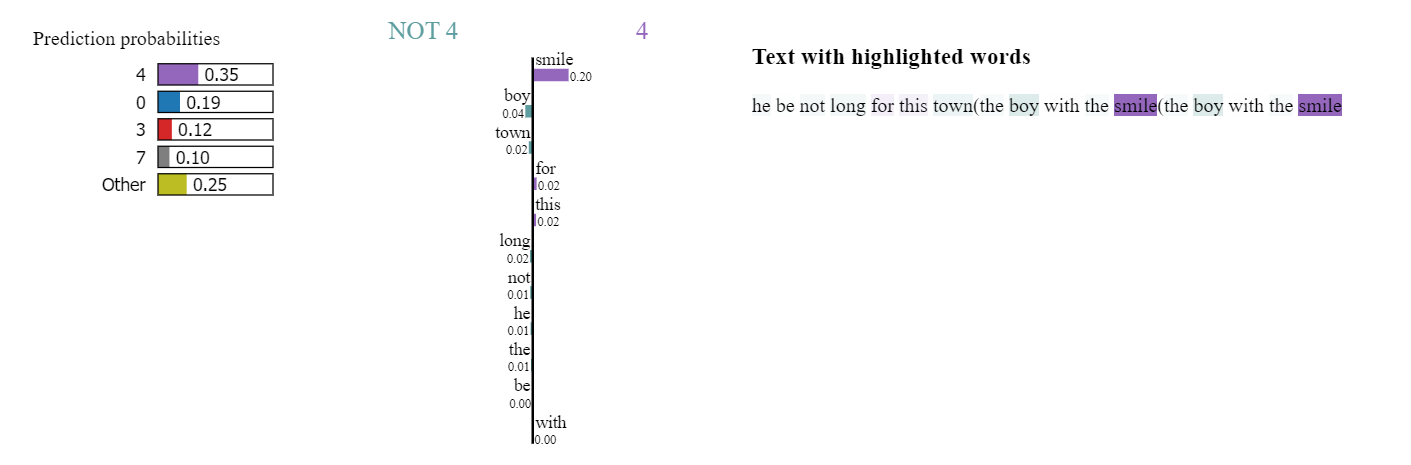
\includegraphics[scale= 0.55]{pictures/expl.png}
    \caption{Explainability - visualization}
    \label{fig:expl}
\end{figure}

The figure above illustrates a prediction where the model assigned the label \texttt{joy} to the stanza under analysis, but the correct label, assigned by the ALBERT model (as mentioned in the \textit{Methods} section), was \texttt{sadness}.
However, the word "smile" which is brighty highlighted, intuitively suggests that "joy" might be a more plausible class for this stanza, even one that ALBERT could reasonably assign. 
This observation raises a critical issue: the transfer learning approach used to create the ground truth appears to have some limitations; in some instances the SVC model assigns a label that seems more contextually appropriate for the stanza, 
yet it differs from the supposedly correct label provided by ALBERT.
